\section{Exercise two}

The Dutch Museum Association wants to keep records of all the Dutch museums and their artworks, as well as keep track of daily visitors and sales.
Each museum is described by a unique name, location (further described by address and city), opening time, closing time, and the average time it takes to visit the whole museum. Opening and closing times are the same every day of the week. 
Every museum is divided into halls, and every hall contains one or more artworks. 
Each hall is described by a unique three-character identifier, title, and one or more types(e.g., sculpture, paintings, etc.). 
Artworks are defined by a unique title, description, and type (same as the hall types). 
Each artwork is produced by only one artist. 
Artists are described by name, surname, date of birth, town of birth, and their life description. 
Visitors buy tickets to visit the museum. 
Each ticket is described by a unique barcode, the number of visitors, and the total price. 
Visitors state the time when they would visit the museum when they buy tickets to allow the museum to keep track of the crowd. 
Museums also include a shop that sells gadgets. 
Each gadget is described by a unique barcode, product name, and price. Visitors buy gadgets at shops.
\begin{enumerate}
    \item The Dutch Museum Association now wants to allow museums to borrow and lend artworks from other museums. 
        They want to keep track of the period each artwork spends in each museum. 
        The latter is agreed on before moving the artwork from one museum to another.
    \item The Dutch Museum Association now wants museums to expand their shops. 
        In particular, now museums will include three different kinds of shops: restaurant, sweets shop, and gadgets shop.
        While the first two shops sell food, the latter sells gadgets.
        Sweet shops only sell sweets. 
        Food is described by the same attributes as gadgets, plus an expiry date.
    \item The Dutch Museum Association wants to model the friendship relationship between the various artists whose artwork are exposed in their museum, considering sculptors and painters only. 
    Furthermore, they made an astounding discovery: painters only befriend other painters and sculptors only befriend other sculptors.
\end{enumerate}
\subsection*{Solution}
The corresponding diagram for the base problem is:
\begin{figure}[H]
    \centering
    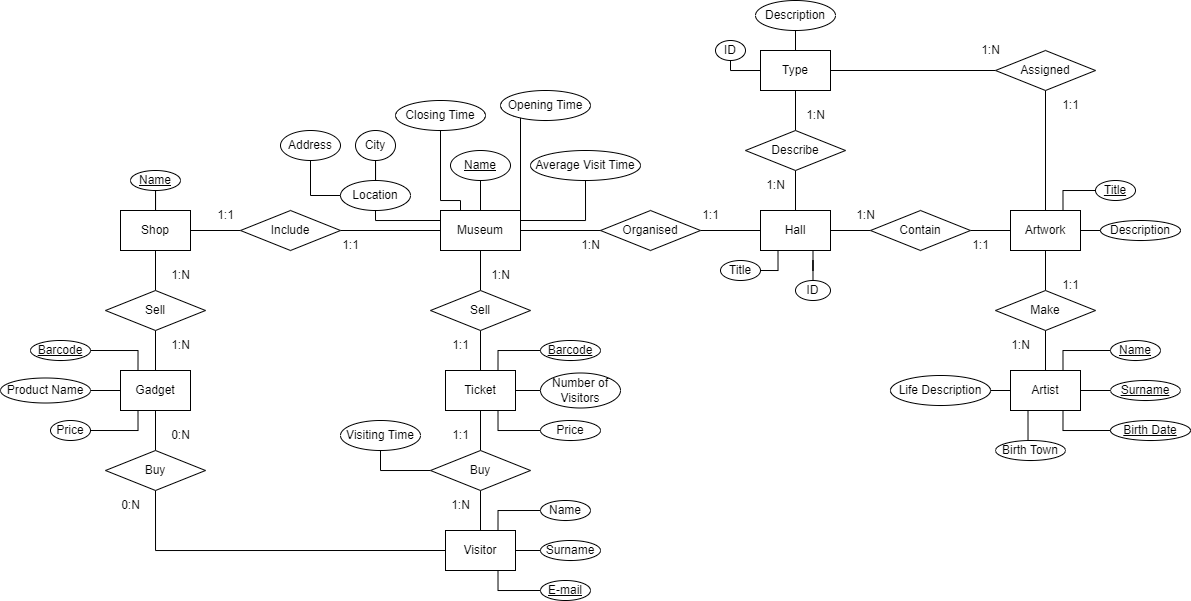
\includegraphics[width=1.00\linewidth]{images/er1.png}
\end{figure}
\begin{enumerate}
    \item The added part is: 
        \begin{figure}[H]
            \centering
            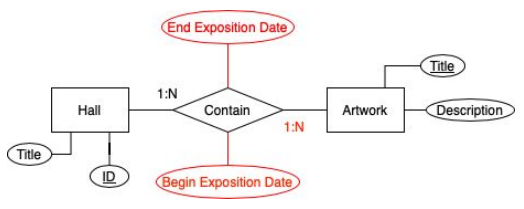
\includegraphics[width=0.75\linewidth]{images/er2.png}
        \end{figure}
    \item The added part is: 
        \begin{figure}[H]
            \centering
            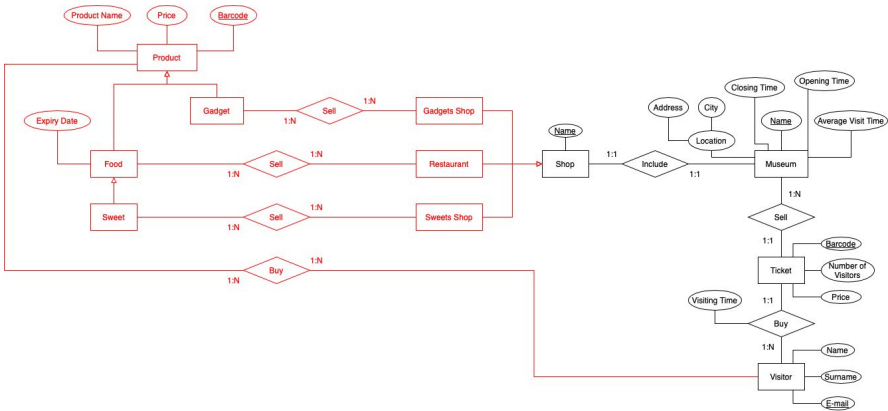
\includegraphics[width=0.75\linewidth]{images/er3.png}
        \end{figure}
    \item The added part is: 
        \begin{figure}[H]
            \centering
            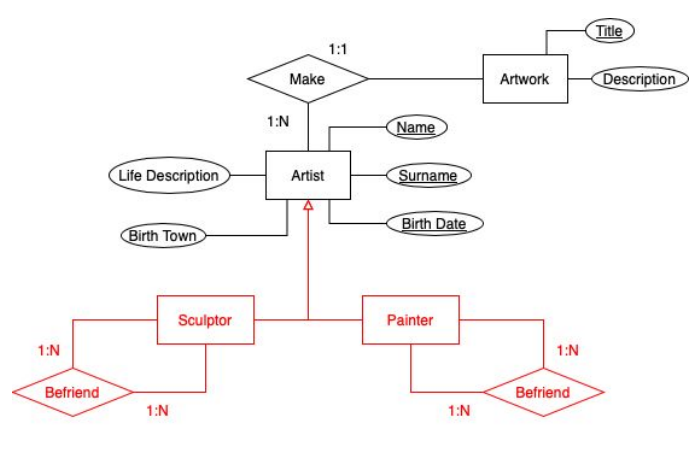
\includegraphics[width=0.75\linewidth]{images/er4.png}
        \end{figure}
\end{enumerate}

